\section{Auswertung}
\subsection{Datenselektion}
Um den Untergrund der Messdaten zu verringern, werden zunächst die Ereignisse aussortiert, bei welchen es sich mit einer hohen Wahrscheinlichkeit nicht um einen $B$-Mesonen Zerfall in drei Kaonen handelt. In den Messdaten findet sich jeweils eine Größe, welche die Wahrscheinlichkeit angibt, dass es sich um ein bestimmtes Sekundärteilchen handelt. Diese beruht auf der Auswertung der Teilchenidentifikationskomponenten des Detektors.

Im Zuge der Selektion muss ein Kompromiss zwischen dem Verwerfen von zu vielen Signalen und dem Einbeziehen zu vieler Hintergrundssignale getroffen werden.
Im Laufe des Versuches sind verschiedene Schnitte ausprobiert worden. Die physikalisch sinnvollsten Ergebnisse werden mit den folgenden Schnitten erzielt:
\begin{itemize}
  \item Das Teilchen soll kein Myon sein: $W_{\mu}=0$.
  \item Die Wahrscheinlichkeit, dass das Teilchen ein Pion ist: $W_{\pi}<0.5$.
  \item Die Wahrscheinlichkeit, dass das Teilchen ein Kaon ist: $W_{K}>0.5$.
\end{itemize}
In den Abbildungen \ref{fig:probK} und \ref{fig:probPi} sind die Wahrscheinlichkeiten $W_{\pi}$ und $W_{K}$ mit den angewendeten Selektierungsschnitten abgebildet. Für $W_{\mu}$ ist dieses nicht nötig, da alle Ereignisse mit einem Myon verworfen werden.
\begin{figure}
  \centering
  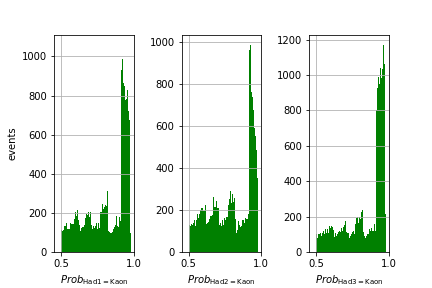
\includegraphics[width=0.7\textwidth]{plots/sim_ProbK_hist.png}
  \caption{Verteilung der Wahrscheinlichkeit, dass es sich bei dem Sekundärteilchen Hadron$_i$ um ein Kaon handelt. Die Achsen sind auf die verwendeten Selektionsgrenzen zugeschnitten.}
  \label{fig:probK}
\end{figure}
\begin{figure}
  \centering
  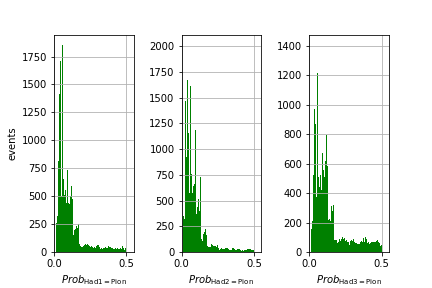
\includegraphics[width=0.7\textwidth]{plots/sim_ProbPi_hist.png}
  \caption{Verteilung der Wahrscheinlichkeit, dass es sich bei dem Sekundärteilchen Hadron$_i$ um ein Pion handelt. Die Achsen sind auf die verwendeten Selektionsgrenzen zugeschnitten.}
  \label{fig:probPi}
\end{figure}
\FloatBarrier
Für die Simulationsdaten muss diese Selektion nicht durchgeführt werden, da nur der Zerfall in drei Kaonen simuliert ist.

\subsection{Energie- und Impulsverteilung der Kaonen}
Für eine Übersicht der im weiteren Verlauf genutzten Variablen werden die Verteilungen der Impulskomponenten beispielhaft für das erste Kaon in Abbildung \ref{fig:Impuls1} dargestellt. Hierzu werden die simulierten Daten verwendet. Diese enthalten weder einen Untergrund, noch sind sie durch Detektionseffekte beeinflusst. Aus diesem Grund lassen sich in ihnen leichter mögliche Fehler der Auswertung erkennen, welche durch unphysikalische Ergebnisse deutlich werden.
\begin{figure}
  \centering
  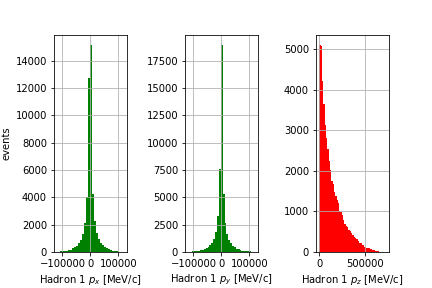
\includegraphics[width=0.7\textwidth]{plots/sim_pall_hist}
  \caption{Verteilung der Impulskomponenten des ersten Hadrons.}
  \label{fig:Impuls1}
\end{figure}
\FloatBarrier
Die Impulskomponenten weisen eine schmale Verteilung um den Wert Null auf.
Die $z$-Komponente des Impulses besitzt nur positive Werte, da diese in Emissionsrichtung des Teilchens liegt. Durch den Boost in Vorwärtsrichtung werden außerdem höhere Impulswerte erreicht, als für die anderen Impulskomponenten.

Über
\begin{align}
  |p|=\sqrt{p_{\mathrm{x}}^2 + p_{\mathrm{y}}^2 + p_{\mathrm{z}}^2 }
  \label{eq:Betrag}
\end{align}
wird der Betrag des Impulses aller drei Kaonen berechnet. Mit Hilfe der
Energie-Impuls-Beziehung \eqref{eq:Epm} und der Kaonmasse aus Tabelle
\ref{tab:quarks} wird die Energie der Kaonen berechnet. Die Energieverteilung
ist in Abbildung \ref{fig:Energie1} zu erkennen.
\begin{figure}
  \centering
  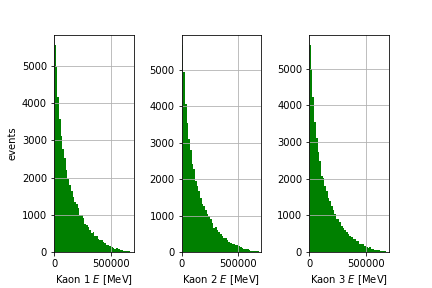
\includegraphics[width=0.7\textwidth]{plots/sim_Eall_hist.png}
  \caption{Energieverteilung der Kaonen.}
  \label{fig:Energie1}
\end{figure}
\FloatBarrier

\subsection{Berechnung der invarianten Masse des B-Mesons}
Die folgenden Auswertungsschritte werden sowohl für die simulierten als auch für die realen Daten durchgeführt.

Für die Berechnung der Energie des $B$-Mesons kann die Energieerhaltung zunutze gemacht werden, sodass sich diese durch die Summierung aller Kaonenenergien ergibt. Für den Impuls des $B$-Mesons werden aufgrund der Impulserhaltung die einzelnen Impulskomponenten der Kaonen aufsummiert und anschließend nach Gleichung \eqref{eq:Betrag} der Impulsbetrag ermittelt.
Die Verteilung der invarianten Masse wird anschließend aus der Energie-Impuls-Beziehung \eqref{eq:Epm} bestimmt und in Abbildung \ref{fig:Minv_sim} für die simulierten Daten und Abbildung \ref{fig:Minv_real} für die Messdaten abgebildet.
\begin{figure}
  \centering
  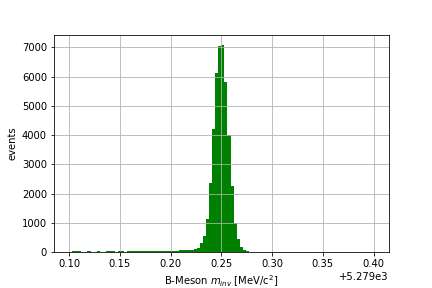
\includegraphics[width=0.7\textwidth]{plots/sim_Bmes_M.png}
  \caption{Verteilung der invarianten Masse des $B$-Mesons für die simulierten Daten.}
  \label{fig:Minv_sim}
\end{figure}
\begin{figure}
  \centering
  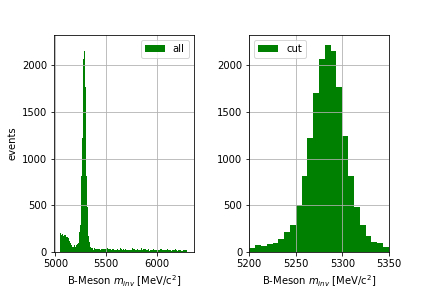
\includegraphics[width=0.7\textwidth]{plots/real_Bmes_M.png}
  \caption{Verteilung der invarianten Masse des $B$-Mesons für die Messwerte. Das rechte Bild ist auf die Grenzen der Massenselektion zugeschnitten.}
  \label{fig:Minv_real}
\end{figure}
\FloatBarrier
In Abbildung \ref{fig:Minv_sim} ist ein scharfer Peak um etwa $\SI{5279.25}{MeV/c^2}$ auszumachen, während die Realdaten eine deutlich breitere Verteilung um diesen Wert aufweisen. Während die Simulation in einer idealen Umgebung abläuft, unterliegen die Realdaten Auflösungseffekten und werden durch einen Untergrund verfälscht. Dieses führt zu einer Normalverteilung der Daten.

Anhand der Massenverteilung wird eine weitere Selektion durchgeführt: Die Daten werden auf Ereignisse mit Primärteilchen der Masse $\SI{5200}{MeV/c^2} < m_{\mathrm{inv}} < \SI{5350}{MeV/c^2} $ zugeschnitten.

\subsection{Globale \textit{CP}-Asymmetrie}
\label{globAsymm}
In diesem Abschnitt werden lediglich die Messdaten verwendet.
Die $CP$-Asymmetrie wird durch den Zusammenhang
\begin{align}
  A_{CP}= \frac{N^{+} - N^{-}}{N^{+} + N^{-}}
  \label{eq:Asymm}
\end{align}
beschrieben, wobei die Größen $N^{+}$ durch die Anzahl von $B^{+}$-Zerfällen und $N^{-}$ durch die Anzahl von $B^{-}$-Zerfällen gegeben sind.
Die Ladung der $B$-Mesonen wird aufgrund der Ladungserhaltung durch das Addieren der drei Kaonenladungen ermittelt. Für die globale $CP$-Asymmetrie wird der Wert
\begin{align*}
  A_{CP} = 0.050 \pm 0.008 \pm 0.010
\end{align*}
berechnet. Die Unsicherheiten setzen sich aus der statistischen Unsicherheit
\begin{align}
  \sigma_{\mathrm{stat}} = \sqrt{\frac{1-A^2}{N^{+} + N^{-}}}
  \label{eq:sigma}
\end{align}
und der systematischen Unsicherheit durch Produktionsasymmetrien zusammen. Letztere entsteht durch eine Asymmetrie der Materie vor der Kollision und hat eine Größe von etwa  $0.01$ \cite{anleitung}.

Durch die Division des Asymmetriewertes mit den Unsicherheiten
\begin{align}
  S_{\mathrm{A}} = \frac{A}{\sqrt{\sigma_{\mathrm{stat}}^2 + \sigma_{\mathrm{syst}}^2}}
  \label{eq:Signifikanz}
\end{align}
ergibt sich eine Signifikanz von $S = 3.978\;\sigma$.

\subsection{Untersuchung auf Zwischenresonanzen mittels Dalitz-Plots}
Zur Untersuchung des $B$-Mesonenzerfalls auf Zwischenresonanzen werden Dalitz-Plots der simulierten und der realen Daten erstellt. Hierbei wird sich zunutze gemacht, dass die Kinematik eines Dreikörperzerfalls durch die Verwendung der Variablen zweier Teilchen vollständig beschrieben werden kann. Im Dalitz-Plot sind die invarianten Massen potentieller Zwischenresonanzen durch eine Kombination der Variablen von zwei verschiedenen Sekundärteilchenkombinationen dargestellt. Die invariante Masse der Zwischenresonanz $ij$ wird über
\begin{align}
  m_{ij} = \sqrt{ E_{ij}^2 - p_{ij}^2}
\end{align}
berechnet, wobei $ E_{ij}$ und $ p_{ij}$ durch eine Addition der Variablen der beiden betrachteten Teilchen ermittelt wird. Die Impulskomponenten müssen hierzu erneut einzelnd addiert werden und der Impulsbetrag der Resonanz nach Gleichung \eqref{eq:Betrag} bestimmt werden.

An dieser Stelle werden die Kombination der Hadronen 1 und 2, sowie 2 und 3 untersucht. Die Verteilung der invarianten Massen $m_{12}$ und $m_{23}$ sind beispielhaft für die simulierten Daten in Abbildung \ref{fig:HistRes} zu sehen.
\begin{figure}
  \centering
  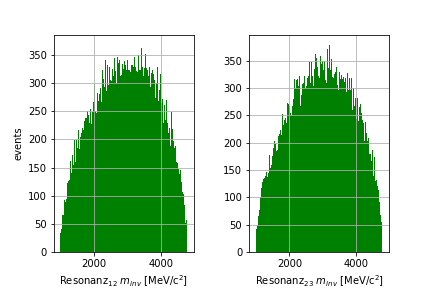
\includegraphics[width=0.7\textwidth]{plots/sim_Xmes_M.png}
  \caption{Verteilung der invarianten Masse der Resonanzen $R_{12}$ und $R_{23}$.}
  \label{fig:HistRes}
\end{figure}
\FloatBarrier
Die invarianten Massen $m_{12}$ und $m_{23}$ werden im Dalitz-Plot gegeneinander aufgetragen, welcher für die simulierten Daten in Abbildung \ref{fig:Dalitz_sim} und für die Messdaten in Abbildung \ref{fig:Dalitz_real} zu erkennen ist.
\begin{figure}
  \centering
  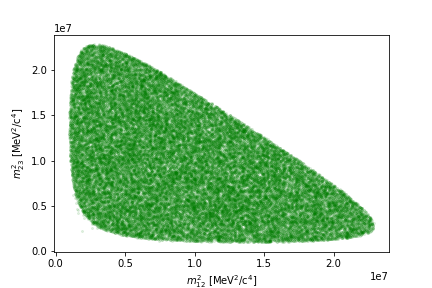
\includegraphics[width=0.7\textwidth]{plots/dalitz_sim.png}
  \caption{Dalitz-Plot der Resonanzen $R_{12}$ und $R_{23}$ für die simulierten Daten für die simulierten Daten.}
  \label{fig:Dalitz_sim}
\end{figure}
\FloatBarrier
\begin{figure}
  \centering
  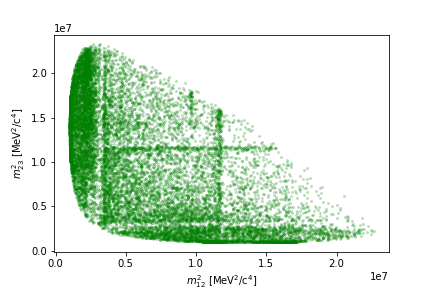
\includegraphics[width=0.7\textwidth]{plots/dalitz_real.png}
  \caption{Dalitz-Plot der Resonanzen $R_{12}$ und $R_{23}$ für die Messdaten.}
  \label{fig:Dalitz_real}
\end{figure}
\FloatBarrier
Zwischenresonanzen zeigen sich im Dalitz-Plot in Form von Bändern an der Stelle der Resonanzteilchenmasse. In den simulierten Daten sind solche Bänder nicht zu erkennen, da in diesen die Simulation des direkten Zerfalles erfolgte. In den Messdaten hingegen werden solche Bänder sichtbar.

Um diese deutlicher darzustellen, werden die Resonanzteilchenmassen umsortiert und erneut ein Dalitz-Plot erstellt. Hierfür wird jeweils die kleinere der Resonanzmassen gegen die dazugehörige Größere aufgetragen. Dadurch wird ein Umklappen des Plottes in der Mitte erreicht, welches zu kompakteren Informationen ohne Verlust der Datenmenge führt. Der umgeklappte Dalitz-Plot ist in Abbildung \ref{fig:Dalitz_klapp} dargestellt.
\begin{figure}
  \centering
  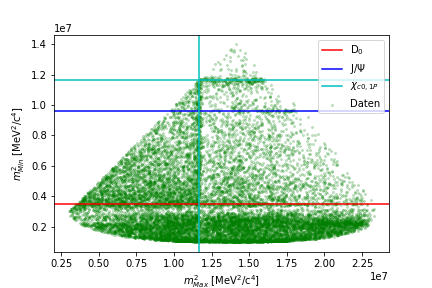
\includegraphics[width=0.7\textwidth]{plots/dalitz_real_MinMax.png}
  \caption{Dalitz-Plot der Resonanzen $R_{12}$ und $R_{23}$, sortiert nach maximaler und minimaler Masse, für die Messdaten. Die Bänder werden über ihre Positionen mit den Resonanzteilchen identifiziert.}
  \label{fig:Dalitz_klapp}
\end{figure}
\FloatBarrier
Anhand der Bänderpositionen können die einzelnen Bänder nun über die Teilchenmassen aus Tabelle \ref{tab:quarks} mit Teilchen identifiziert werden. Es lassen sich die Resonanzen $D_0$, $J/\Psi$ und $\Chi_{c0}$ ausmachen, welche alle ein $c$-Quark enthalten.
In der CKM-Matrix findet sich in dem Eintrag $V_{\mathrm{cb}}$ kein Hinweis auf $CP$-Verletzung.
Daher werden sie aus den Daten entfernt. Hierzu werden die Daten verworfen, deren Resonanzmasse im Bereich eines Bandes liegt. Der selektierte Dalitz-Plot ist Abbildung \ref{fig:Dalitz_sel} zu entnehmen.
\begin{figure}
  \centering
  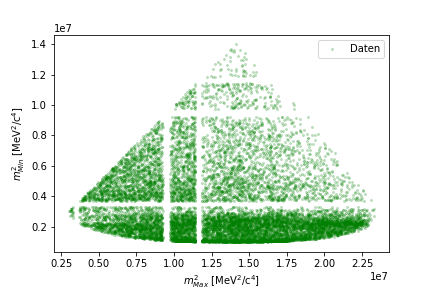
\includegraphics[width=0.7\textwidth]{plots/dalitz_real_MinMax_ohnec.png}
  \caption{Dalitz-Plot der Resonanzen $R_{12}$ und $R_{23}$, sortiert nach maximaler und minimaler Masse, für die Messdaten mit entfernten Resonanzen.}
  \label{fig:Dalitz_sel}
\end{figure}
\FloatBarrier

\subsection{Lokale \textit{CP}-Asymmetrie}
Die $CP$-Asymmetrie kann aufgrund von Zerfällen über verschiedene Resonanzen über den Phasenraum unterschiedliche Werte und Größenordnungen annehmen. Dieser Effekt soll nun berücksichtigt werden.

Da eine $CP$-Symmetrie aus der Interferenz von Zerfällen unterschiedlicher Resonanzen entsteht, wird diese durch Unterschiede in den Dalitz-Plots von $B^{+}$ und $B^{-}$ deutlich. Aus diesem Grund werden in Abbildung \ref{fig:DalitzPM} die einzelnen Dalitz-Plots von $B^{+}$ und $B^{-}$ dargestellt und die Asymmetrie nach Gleichung \eqref{eq:Asymm} zwischen den Plots in jedem Bin ermittelt. Hiezu wurde ein relativ grobes Binning verwendet, um eine ausreichend hohe Menge an Daten in jedem Bin zu erreichen und somit den statistischen Fehler zu minimieren. Die Asymmetrie der Dalitz-Plots ist in Abbildung \ref{fig:DalitzDiff} zu sehen.
\begin{figure}
  \centering
  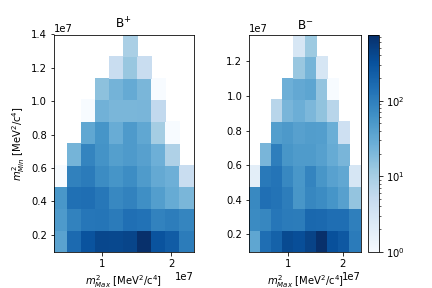
\includegraphics[width=0.7\textwidth]{plots/Bp_Bm_Dalitz.png}
  \caption{Dalitz-Plot der Resonanzen $R_{12}$ und $R_{23}$, sortiert nach maximaler und minimaler Masse, von $B^{+}$ und $B^{-}$ für die Messdaten.}
  \label{fig:DalitzPM}
\end{figure}
\FloatBarrier
\begin{figure}
  \centering
  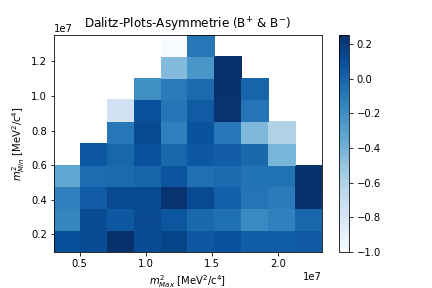
\includegraphics[width=0.7\textwidth]{plots/Asymm_Dalitz.png}
  \caption{Asymmetrie der Dalitz-Plots von $B^{+}$ und $B^{-}$ für die Resonanzen $R_{12}$ und $R_{23}$ der Messdaten, sortiert nach maximaler und minimaler Masse.}
  \label{fig:DalitzDiff}
\end{figure}
\FloatBarrier
Die statistische Unsicherheit der Asymmetrie wird ebenfalls für jeden Bin nach Gleichung \eqref{eq:sigma} bestimmt und in Abbildung \ref{fig:DalitzAsymmUnsi} dargestellt.
\begin{figure}
  \centering
  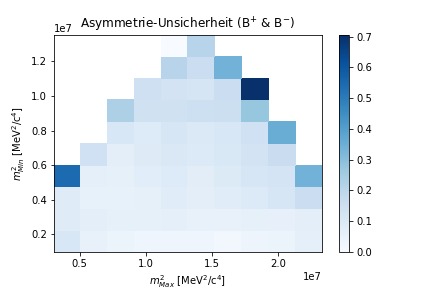
\includegraphics[width=0.7\textwidth]{plots/Asymm_Fehler_Dalitz.png}
  \caption{Statistische Unsicherheit der Asymmetrie der Dalitz-Plots von $B^{+}$ und $B^{-}$ für die Resonanzen $R_{12}$ und $R_{23}$ der Messdaten, sortiert nach maximaler und minimaler Masse.}
  \label{fig:DalitzAsymmUnsi}
\end{figure}
\FloatBarrier
Besonders hohe Unsicherheiten sind an den Rändern des Plottes zu erkennen. Um ihren Einfluss auf die Asymmetriewerte auszumachen, wird die Signifikanz der $CP$-Asymmetrie nach Gleichung \eqref{eq:Signifikanz} in jedem Bin bestimmt. Diese ist in Abbildung \ref{fig:DalitzSign} zu sehen.
\begin{figure}
  \centering
  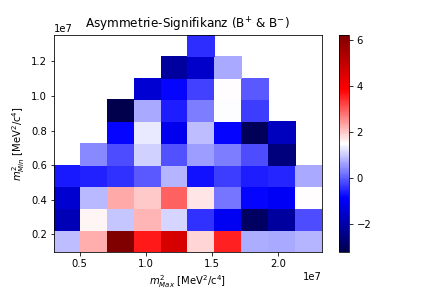
\includegraphics[width=0.7\textwidth]{plots/Asymm_Sig_Dalitz.png}
  \caption{Signifikanz der Asymmetrie der Dalitz-Plots von $B^{+}$ und $B^{-}$ für die Resonanzen $R_{12}$ und $R_{23}$ der Messdaten, sortiert nach maximaler und minimaler Masse.}
  \label{fig:DalitzSign}
\end{figure}
\FloatBarrier
Liegt die Signifikanz einer Messung in einem Bereich oberhalb von $3\;\sigma$ wird in der Teilchenphysik von einem Hinweis auf eine Entdeckung gesprochen. Ein zusammenhängender Bereich, für den dieses zutrifft, ist in Abbildung \ref{fig:DalitzSign} durch die grünen Linien markiert.

Dieser Bereich wird nun genauer untersucht. Dafür werden die Verteilungen der invarianten Massen des $B^{+}$- und $B^{-}$-Mesons in diesem relevanten Bereich in Abbildung \ref{fig:AsymmMassen} dargestellt.
\begin{figure}
  \centering
  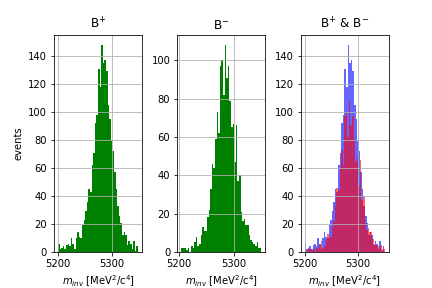
\includegraphics[width=0.7\textwidth]{plots/Bp_Bm_invarianteMasse.png}
  \caption{Verteilung der invarianten Massen des $B^{+}$- und $B^{-}$-Mesons im Bereich einer hohen Signifikanz für $CP$-Asymmetrie. Im rechten Plot stellt die Farbe rot die Verteilung des $B^{-}$-Mesons dar und blau die Verteilung des $B^{+}$-Mesons.}
  \label{fig:AsymmMassen}
\end{figure}
\FloatBarrier
Im übereinandergelegten Histogramm ist deutlich ein vermehrtes Vorkommen des $B^{+}$- gegenüber dem $B^{-}$-Meson auszumachen.

Für den Mittelwert der Signifikanz der $CP$-Asymmetrie im relevanten Bereich wird zuletzt analog zu Abschnitt \ref{globAsymm} der Wert
\begin{align}
  S_{CP} = 7.89\;\sigma
\end{align}
ermittelt.
